\documentclass{IEEEtran}
\usepackage{cite}
\usepackage{amsmath,amssymb,amsfonts}
\usepackage{graphicx}
\usepackage{textcomp,nicefrac}

%-----------------------------------------------------------------------------------
% reduce margins
\usepackage[a4paper,top=2cm,bottom=1.5cm,left=1.0cm,right=1.0cm]{geometry}

\usepackage{algorithmicx}
\usepackage{algpseudocode}

% define float env for algorithm
\usepackage{float}
\floatstyle{ruled}
\newfloat{algorithm}{h}{loa}
\floatname{algorithm}{Algorithm}

% custom definitions
\DeclareMathOperator{\proj}{proj}
\DeclareMathOperator{\prox}{prox}
\DeclareMathOperator*{\argmin}{arg\,min}
%-----------------------------------------------------------------------------------

\usepackage[colorinlistoftodos,prependcaption,textsize=footnotesize]{todonotes}

%-----------------------------------------------------------------------------------

\def\BibTeX{{\rm B\kern-.05em{\sc i\kern-.025em b}\kern-.08em
T\kern-.1667em\lower.7ex\hbox{E}\kern-.125emX}}
\markboth{IEEE NSS/MIC conference 2021}
{Schramm \MakeLowercase{\textit{et al.}}: List-mode SPDHG}


\begin{document}
\title{\vspace{-0.5cm}Fast list-mode reconstruction of sparse TOF PET data with non-smooth priors} 
\author{Georg Schramm and Martin Holler\vspace{-1cm}
\thanks{G.S. is with the Department of Imaging and Pathology, Division of Nuclear Medicine,
KU Leuven, Belgium, (e-mail: georg.schramm@kuleuven.be).}
\thanks{M.H. is with the Institute of Mathematics and Scientific Computing, 
University of Graz, Austria}
}

\maketitle

\begin{abstract}
In this work, we propose and analyze a list-mode version of the stochastic primal-dual hybrid gradient
(SPDHG) algorithm for image reconstruction from TOF PET data using subsets and non-smooth priors. 
By strongly exploiting sparsity in the TOF PET data, our proposed algorithm substantially reduces both memory requirements and computation time. 
To study the behavior of the proposed algorithm in detail, its performance 
is investigated based on simulated 2D TOF data using a brain-like software phantom.

We find that our listmode-version of SPDHG converges essentially as fast the original version,
which will lead to a substantial improvement in the time needed for a reconstruction
of real 3D TOF PET data.
However, as with the original algorithm, a careful choice of the ratio of the primal and dual step sizes, 
depending on the magnitude of the image to be reconstructed, is crucial to obtain fast convergence.
\end{abstract}

\begin{IEEEkeywords}
Positron emission tomography, Reconstruction algorithms
\end{IEEEkeywords}

\section{Introduction}

Recently, Chambolle et al. \cite{Chambolle2018} and  Ehrhardt et al. \cite{Ehrhardt2019} introduced 
the stochastic primal-dual hybrid gradient (SPDHG) algorithm which is a provably convergent algorithm
that allows to solve the sinogram-based PET reconstruction problem including many non-smooth priors with
only a few iterations.
As discussed in Remark 2 of \cite{Ehrhardt2019}, a potential drawback of SPDHG is that it requires
to keep at least one more complete (TOF) sinogram ($y$) in memory. 
%Moreover, if the proposed preconditioning is used, a second complete (TOF) sinogram
%(the sequence of step sizes $(S_i)_{i=1}^n$) needs to be stored.
In general, this is less of a problem for static single-bed non-TOF PET data, where sinogram sizes
are relatively small.
However, for simultaneous multi-bed, dynamic or TOF PET data, the size of complete sinograms
can be become problematic, especially when using GPUs.
For example, for modern PET TOF scanners with 25\,cm axial FOV and a TOF resolution of ca. 400\,ps, 
a complete unmashed TOF sinogram in single precision for one bed position 
has approximately $4.4\cdot10^9$ data bins, requiring ca. 17\,GB of memory.
Note that the memory required to store a complete TOF sinogram and its sparsity will further 
increase with better TOF resolution.
Due to the large number of data bins and the limitations in injected dose and acquisition time,
modern TOF sinograms are usually very sparse, meaning that in most data bins no data is
acquired.
E.g., for a typical 3\,min-per-bed-position whole-body FDG scan with an injected dose 
of around 200\,MBq acquired 60\,min p.i. on a state-of-the-art TOF PET/MR scanner, 
more than 95\% of the data (TOF sinogram) bins are empty.
For short early frames in dynamic brain scans, this fraction is even higher.
And even for ``high count'' late static 20\,min FDG brain scans with an injected dose of 150\,MBq
acquired 60\,min p.i., still around 70\% of the data bins are empty.
Due to the very sparse nature of the acquired data, list-mode (event-by-event) type
reconstruction algorithms - such as e.g. list-mode OSEM - are computationally more efficient
than algorithms working with binned data (sinograms).
For example, with a high count (1e8 events) and a medium count (1e7 events) acquisition, 
a complete forward and back projection in list-mode is faster by roughly a factor of 2 and 20,
respectively, compared to a sinogram projection for state of the art TOF PET scanner 
with a TOF resolution of ca. 400\,ps.
Motivated by this finding, 
in this work we present an adaption of the SPDHG algorithm that maintains global convergence guarantees while allowing to work only with list-mode data during iterations.
With this, in particular, the iterations of our algorithm can completely ignore sinogram bins where no events where detected.

%the aim of this work is to present a modification of the convergent 
%SPDHG algorithm that allows efficient processing of PET data in list-mode instead of sinograms.

\section{Methods}

In this work, we focus on time-of-flight (TOF) PET reconstruction using TV regularization, 
noting, however, that generalizations to other non-smooth priors as mentioned above are possible 
within the same framework. 
The TV regularized TOF PET reconstruction method requires to solve the optimization problem
%
\begin{equation} \label{eq:main_minimization_problem}
\argmin _{x\geq 0} \sum_j (Px)_j -  d_j \log \left( (Px)_ j + s_j \right) + \beta \, \|\nabla x\|_{1},
\end{equation}
%
where $x$ is the PET image to be reconstructed, $P$ is the (sinogram) TOF forward projector including 
the effects of attenuation and normalization, $d$ are the acquired prompt TOF coincidences 
(the emission sinogram), and $s$ are additive contaminations including random and scattered coincidences.
The operator $\nabla$ is the gradient operator, $\|\nabla u \|_1$ is sum over all entries of the 
pointwise Euclidean norm of $\nabla u$, and $\beta$ is a scalar controlling the level of regularization.

To work with the emission data in list-mode format, given a list $N$ of detected events $e \in N$, we introduce the list-mode forward operator $P_N$ mapping image data $x$ to a data-vector of dimension $|N|$ via
\[ (P_Nx)_e  = P_{j_e}x , \text{ for each }e \in N,\]
where $j_e$ is the sinogram-bin in which event $e$ was detected.
% and $\mu_{e}$ is the total number of events in list $N$ detected in the bin $j_e$.%, i.e., if a certain event detected in bin $i$ is present $n$ times in the event list $N$, then $\mu_e = n$.

Using this list-mode forward operator $P_N$, and taking special care of sinogram bins where no events where detected, we can equivalently reformulate problem \eqref{eq:main_minimization_problem} in terms of the list-mode operator $P_N$ and list mode data. Building on this, we propose the list-mode SPDHG (LM-SPDHG) as shown
in Algorithm~\ref{alg:lmspdhg} algorithm for the numerical solution of \eqref{eq:main_minimization_problem}

Note that the main advantage of our algorithm, compared to a sinogram-based version, is that in every update involving the PET data, only a list-mode forward and back projection of
a subset of the list-mode data is needed. Beyond that, only one additional array with the same length
as the event list need to be kept in memory during the iterations. 

In the pre-processing step 2, the event counts $\mu_e$ need to be calculated once for every event in $N$. Here, $\mu_{e}$ is the total number of events in list $N$ detected in the sinogram-bin $j_e$ where the event $e$ was recorded.
Note that in step 5, the images $\bar{z}$ and $z$ need to be initialized with the adjoint sinogram
operator applied on the sinogram $y$ which is a sinogram that is one in all bins where no data was
recorded and zero else. The sinogram $y$ does not need to be kept in memory after this step.

To compare the convergence of SPDHG and LM-SPDHG, we performed reconstructions of simulated
TOF PET data from a virtual 2D scanner mimicking the TOF resolution (ca. 400\,ps FWHM) and 
geometry of one ring (direct plane) of the GE SIGNA PET/MR (sinogram dimension: 
357 radial bins, 224 projection angles, 27 TOF bins).
A software brain phantom with a typical gray to white matter contrast of 4:1 was created
based on the brainweb phantom and used to generate simulated data including the effects
of attenuation and flat contamination (scattered) coincidences
with a simulated scatter fraction of 16\%.
Noisy simulated prompt emission TOF sinograms and corresponding list-mode data sets 
were generated for $10^6$ counts.

The simulated data were reconstructed with SPDHG and LM-SPDHG using 100 iterations, 56 subsets,
and a fixed level regularization $\beta = 0.002$ and different step size ratios.
As in \cite{Ehrhardt2019}, convergence was monitored by tracking the relative cost function
\[ c_\text{rel}(x) = (c(x) - c(x^*)) / (c(x^0) - c(x^*)). \]
compared to an approximate minimizer $x^*$,
which was calculated using the deterministic (sinogram) PDHG with 10000 iterations without subsets.


%-----------------------------------------------------------------------------
\begin{algorithm}[t]
\begin{algorithmic}[1]
\footnotesize
\State \textbf{Input} event list $N$
\State \textbf{Calculate} event counts $\mu_e$ for each e in $N$ (see text)
\State \textbf{Split} event list $N$ into $m$ sublists $N_i$
\State \textbf{Initialize} $x,(S_i)_i,T,(p_i)_i,g$
\State \textbf{Preprocessing} $\overline{z} = z = P^T y$ (see text)
\State \textbf{Initialize} $m$ sub lists $l_{N_i}$ with 0s
\Repeat
	\State $x = \proj_{\geq 0} (x - T \overline{z})$
	\State Select $i \in \{1,\ldots,m+1\}$ randomly accord. to $(p_i)_i$
  \If{$i \leq m$}
	  \State $l_{N_i}^+ \gets \prox_{D^*}^{S_i} \left( l_{N_i} + S_i \left(P_{N_i} x + s_{N_i} \right) \right)$
	  \State $\delta z \gets P_{N_i}^T \left(\frac{l_{N_i}^+ - l_{N_i}}{\mu_{N_i}}\right)$
	  \State $l_{N_i} \gets l_{N_i}^+$
  \Else
	  \State $g^+ \gets \prox_{||\cdot||^*}^{S_i} \left( g + S_i \nabla x \right)$
	  \State $\delta z \gets \nabla^T \left(g^+ - g\right)$
	  \State $g \gets g^+$
  \EndIf
	\State $z \gets z + \delta z$
	\State $\overline{z} \gets  z + (\delta z/p_i)$
\Until{stopping criterion fulfilled}
\State \Return{$x$}
%\EndFunction
\end{algorithmic}
\caption{LM-SPDHG for PET reconstruction}
\label{alg:lmspdhg}
\end{algorithm}

%-----------------------------------------------------------------------------

\section{Results}

As shown in Figure~\ref{fig:recons}, the reconstructions obtained with (sinogram) SPDHG and LM-SPDHG
are very similar and very close to the reference reconstruction.
Figure~\ref{fig:cost} demonstrates that the convergence of (sinogram) SPDHG and
LM-SPDHG is also very similar. In the early iterations, the convergence of LM-SPDHG is a bit slower, but
at late iterations slightly lower values of the cost function are obtained with LM-SPDHG.
Both figures show again that the choice of ratio between the step sizes $S_i$ and $T$ has
a strong influence on the convergence speed.

\begin{figure}[t]
\centerline{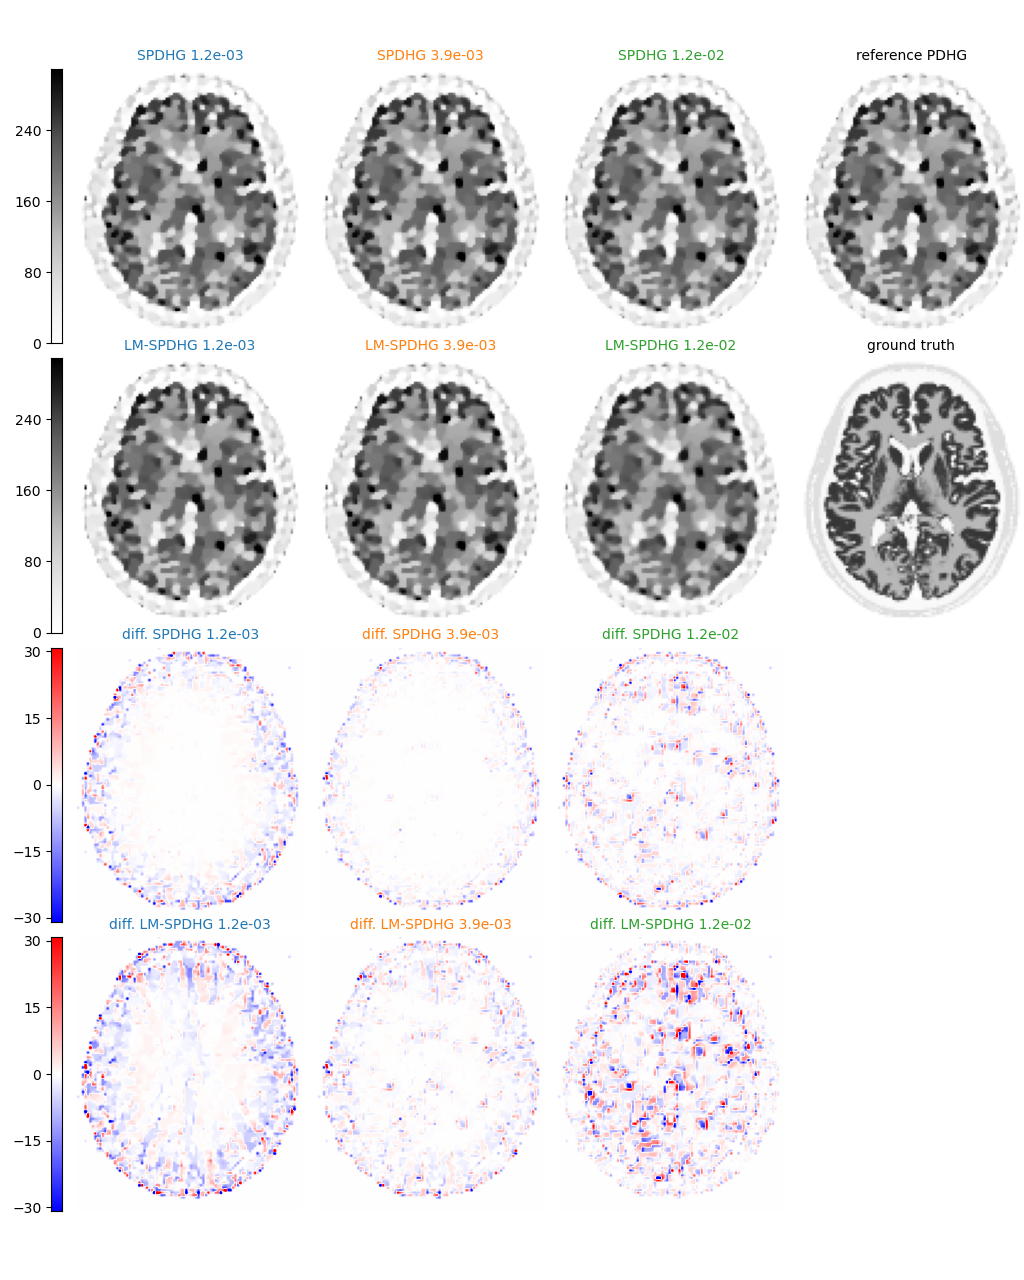
\includegraphics[width=1.0\columnwidth]{./figs/brain2d_counts_1.0E+06_beta_2.0E-03_niter_10000_100_nsub_56_precond_False.png}}
\caption{Reconstructions using 100 iterations and 56 subsets with (sinogram) SPDHG (top row) and 
LM-SPDHG (2nd row) for three different step size ratios. 
There reference PDHG reconstruction without subsets and 10000 iterations and
the ground truth image are shown in the last column. 
The two bottom rows show the difference of the SPHDG and LM-SPDHG reconstructions with respect
to the reference PDHG reconstruction, respectively.}
\label{fig:recons}
\end{figure}

\begin{figure}[t]
\centerline{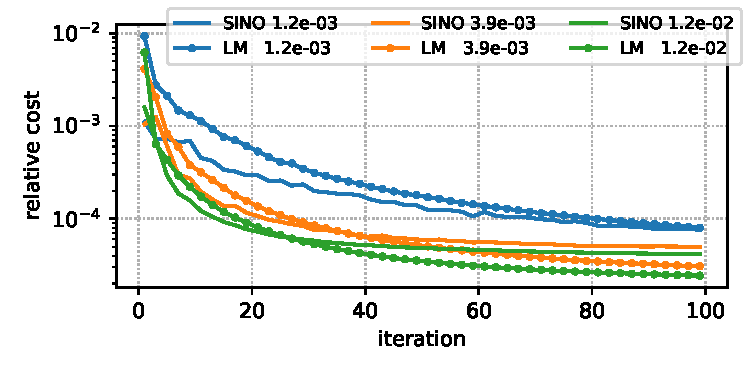
\includegraphics[width=0.8\columnwidth]{./figs/brain2d_counts_1.0E+06_beta_2.0E-03_niter_10000_100_nsub_56_precond_False_metrics.pdf}}
\caption{Convergence of relative cost for SPDHG (dashed line) and LM-SPDHG (triangles) 
for for three different step size ratios (colors).}
\label{fig:cost}
\end{figure}

%-----------------------------------------------------------------------------

\section{Discussion}

The proposed LM-SPDHG algorithm allows for  iterative PET reconstruction of list-mode
data with subsets and non-smooth priors.
For sparse TOF PET data that results in substantially reduced memory requirement during
the iterations and improved computational efficiency depending on the number of acquired
events.
However, preprocessing steps 2 and 5 pose a computational overhead. 
Before the iterations, the event counts $\mu_e$ for every bin present in the event list
have to be calculated and stored.
Moreover, the variables $z$ and $\bar{z}$ have to be initialized with a sinogram
backprojection of $y$ which is in a way ``similar'' to the calcuation of the sensitivity
image in list-mode OS-MLEM.
Nevertheless, for real 3D TOF PET data at usual count levels (especially in shorter frames), one can
expect the computation time and memory requirement of the proposed LM-SPDHG algorithm to be significantly reduced compared to standard sinogram-based SPDHG.
In the future, we also plan to compare the results against the EM-TV algorithms that also
allows list-mode processing.

%-----------------------------------------------------------------------------
%-----------------------------------------------------------------------------

\begin{thebibliography}{00}
\bibitem{Chambolle2018}A. Chambolle, M. J. Ehrhardt, P. Richtarik, et al. 
``Stochastic primal-dual hybrid gradient algorithm with arbitrary sampling and imaging
applications``. 
\textit{SIAM Journal on Optimization}, vol. 28, no. 4, 2018

\bibitem{Ehrhardt2019} M. J. Ehrhardt, P. Markiewicz, and C. B. Sch\"onlieb. 
``Faster PET reconstruction with non-smooth priors by randomization and preconditioning``. 
\textit{Phys Med Biol}, vol. 64, no. 22, 2019
\end{thebibliography}


\end{document}
